% Created 2023-04-29 Sat 15:29
% Intended LaTeX compiler: pdflatex
\documentclass[11pt]{article}
\usepackage[utf8]{inputenc}
\usepackage[T1]{fontenc}
\usepackage{graphicx}
\usepackage{longtable}
\usepackage{wrapfig}
\usepackage{rotating}
\usepackage[normalem]{ulem}
\usepackage{amsmath}
\usepackage{amssymb}
\usepackage{capt-of}
\usepackage{hyperref}
\author{Yusheng Zhao}
\date{\today}
\title{Assignment 3}
\hypersetup{
 pdfauthor={Yusheng Zhao},
 pdftitle={Assignment 3},
 pdfkeywords={},
 pdfsubject={},
 pdfcreator={Emacs 28.2 (Org mode 9.6.1)}, 
 pdflang={English}}
\begin{document}

\maketitle


\section{Problem 1}
\label{sec:org81370df}
From statistical mechanics, we know the following rule. When there is a phase
change, some function related to the structure of the system will change
abruptly. More specifically, you could calculate \textbf{RMSD} for the system under
investigation. Over time, you should see a discontinuity in the plot of time
versus \textbf{RMSD}. That's when a phase change occurred.

A plot may look something like this.

\begin{center}
\includegraphics[width=.9\linewidth]{../../../notes/imgs/pdfs/Problem_1/20230429-112158_Screenshot 2023-04-29 at 11.21.55.png}
\end{center}

\section{Problem 2}
\label{sec:org269a7c0}
In a folded protein, I expect to find hydrophobic amino acids in the \textbf{innerds}
of the structure. Conversely, I expect to find hydrophilic amino acids on the
\textbf{outside} of the folded protein. This is basically due to the need to minimize
energy in the folded state of a protein.

\begin{itemize}
\item Hydrophobic Amino Acid: Alanine
\item Hydrophilic Amino Acid: Aspartic Acid
\item I have illustrated the protein: BARNASE MUTANT WITH ILE 88 REPLACED BY ALA
(1BRJ). In addition, I illustrated the hydrophobic amino acid, Alanine, as
balls. I also illustrated the hydrophilic amino acid, Aspartic Acid, as
surface.
\end{itemize}

\begin{center}
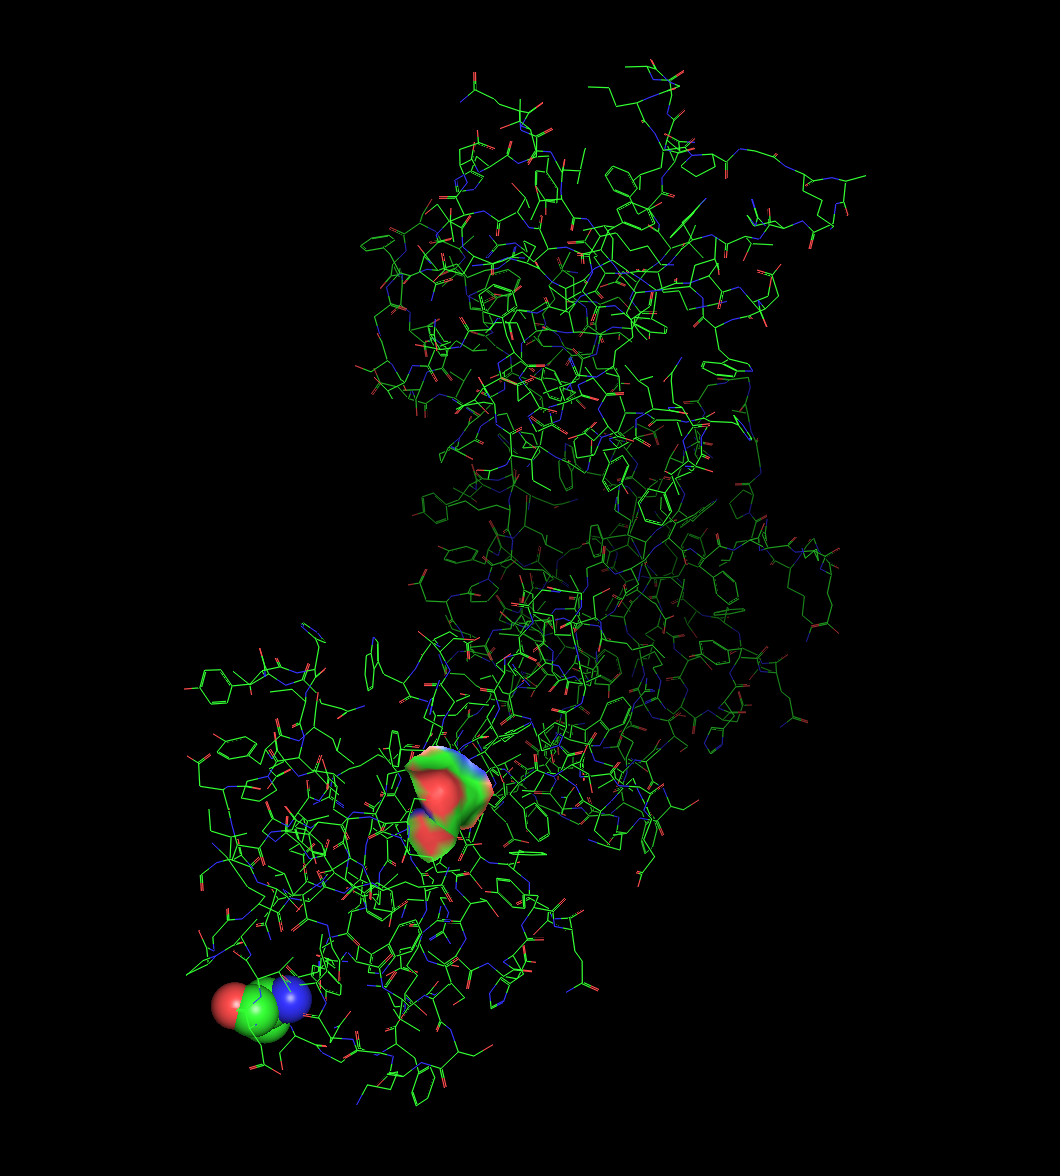
\includegraphics[width=.9\linewidth]{./protein.png}
\end{center}

\section{Problem 3}
\label{sec:orgafb7d97}
Professor Chu gave a very good flow chart on 27 of Week 10 slides. I could not
have done better and don't feel like robbing him of his work. Therefore, the
flow chart will be omitted. But the following steps are summarized from that
lecture note.
\subsection{Structure Conversion and Topology}
\label{sec:org2662723}
\begin{itemize}
\item Load PDB file
\item Choose a certain force field
\item Generate topology file with \texttt{pdb2gmx} command
\end{itemize}

\subsection{Define Periodic Boundary Condition}
\label{sec:orgc2380db}
\begin{itemize}
\item Define the box for PBC
\item Limit minimal interaction distance
\end{itemize}

\subsection{Add Solvent and Ion}
\label{sec:org7acd20e}
\begin{itemize}
\item Add solvent explicitly with \texttt{solvate} command
\item Replace some solvent molecule with ions to make system charge neutral.
\end{itemize}

\subsection{Energy Minimization}
\label{sec:orged4632b}
\begin{itemize}
\item Equilabrate the system by performing energy minimization on the system.
\item It's necessary because the added solvent might have created a large repulsion
on the system that will ruin the MD simulation process.
\end{itemize}

\subsection{NVT Ensemble Equilibration}
\label{sec:orga9dd545}
\begin{itemize}
\item Couple system to heat bath and equilibrate the temperature of the system to
desired value.
\item Run simulation to allow for equilibration.
\end{itemize}

\subsection{NPT Ensemble Equilibration}
\label{sec:org7345c40}
\begin{itemize}
\item Turn on the pressure coupling. Allow for the system to equilibrate.
\item The end of simulation. Get ready to analyze result.
\end{itemize}

\section{Problem 4}
\label{sec:orgfad0327}
\subsection{A}
\label{sec:orgf1e38f0}
In general, we cannot \textbf{accurately} estimate the binding affinity. By definition,
binding affinity is the concentration of ligand where half of protein is bounded
with the ligand. It is statistical average value. Therefore, we need a
statistical ensemble to accurately estimate it. For a single simulation we might
be able to rely on ergodicity. However, we don't know how long the simulation
ran. So ergodicity condition may not apply. Single trial may not represent all
possible starting configuration of the drug. Furthermore, random fluctuation
during the simulation may render the simulation result not representative.

\subsection{B}
\label{sec:orgf70085f}
According to the lecture note, I propose to calculate the binding affinity from
the free energy calculation. Free energy calculation will be carried out using
the Free Energy Perturbation (FEP) method and alchemical method to speed things
up.

Firstly, we add a non-existing force onto the drug molecule to slowly drive it
to bind with the target protein. Then, we divide the process of evolving from
the un-binded state to the binded state into many small steps where the initial
and final configuration of the drug and protein within each step is not too
different. This is a perturbation. Free energy difference of between the
perturbed state and un-perturbed state is easily calculable.

In case of a driving process being extremely long with the added force, we could
deploy alchemical method to directly induce a mutation to speed up the process.

Lastly, the free energy difference along the entire process is accumulated to
get the free energy difference between the un-binded and binded state. The
binding affinity could be derived from the free energy difference.
\end{document}